\newpage

\subsection{QuizziPedia::Front-End::Templates}

	\label{QuizziPedia::Front-End::Templates}
	\ref{QuizziPedia::Front-End::Templates}
	\begin{figure}[h]
		\centering
		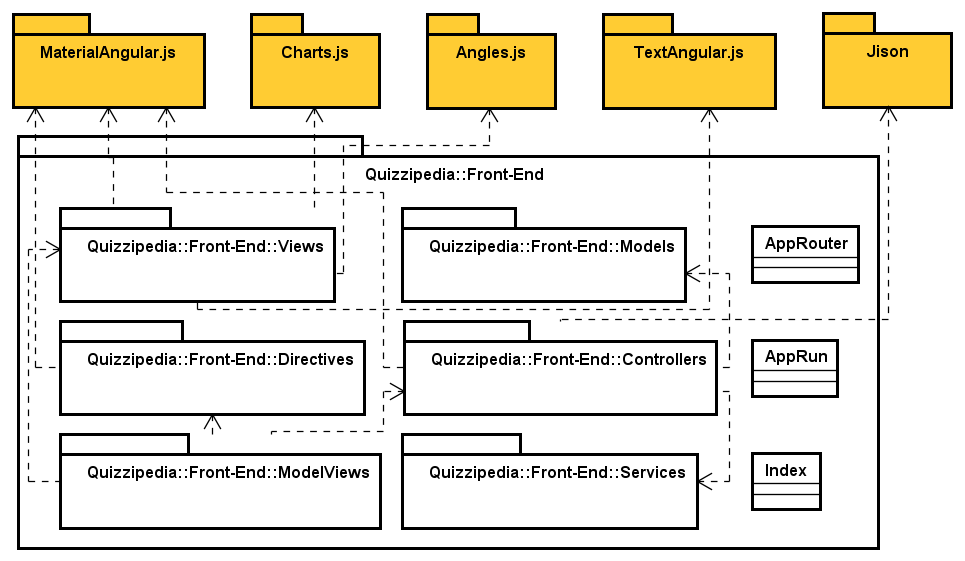
\includegraphics[scale=0.5,keepaspectratio]{UML/Classi/Package/QuizziPedia_Front-end.png}
		\caption{QuizziPedia::Front-End::Templates}
	\end{figure}
	
	\subsubsection{Informazioni generali}
		\begin{itemize}
			\item \textbf{Descrizione}: ;
			\item \textbf{Padre}: ;
			\item \textbf{Iterazioni con altri componenti}: ;
		\end{itemize}

	\subsubsection{Classi}
		\paragraph{QuizziPedia::Front-End::Template::AllenamentoSetUpTemplate}
		
				\label{QuizziPedia::Front-End::Templates::AllenamentoSetUpTemplate}
				\ref{QuizziPedia::Front-End::Templates::AllenamentoSetUpTemplate}
				\begin{figure}[h]
					\centering
					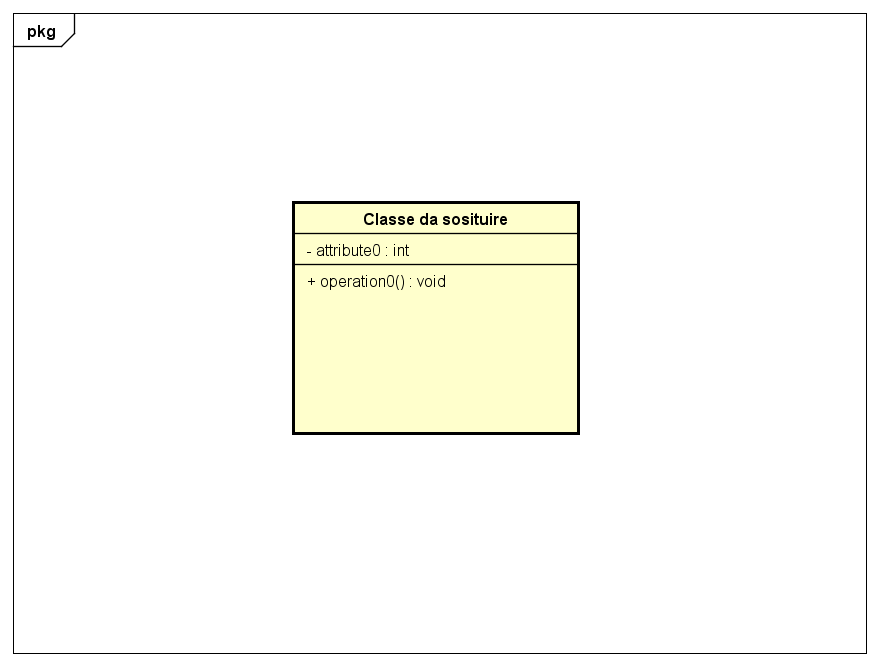
\includegraphics[scale=0.5,keepaspectratio]{UML/Classi/Classi/Temporanea.png}
					\caption{QuizziPedia::Front-End::Templates::AllenamentoSetUpTemplate}
				\end{figure}
						
			\begin{itemize}
				\item \textbf{Descrizione}: ;
				\item \textbf{Utilizzo}: ;
				\item \textbf{Relazioni con altre classi}: 
					\begin{itemize}
						\item ;
					\end{itemize}
				\item \textbf{Attributi}: 
					\begin{itemize}
						\item ;
					\end{itemize}
				\item \textbf{Metodi}: 
					\begin{itemize}
						\item ;
					\end{itemize}
			\end{itemize}

		\paragraph{QuizziPedia::Front-End::Template::HeaderRispostaDomandeTemplate}
		
				\label{QuizziPedia::Front-End::Templates::HeaderRispostaDomandeTemplate}
				\ref{QuizziPedia::Front-End::Templates::HeaderRispostaDomandeTemplate}
				\begin{figure}[h]
					\centering
					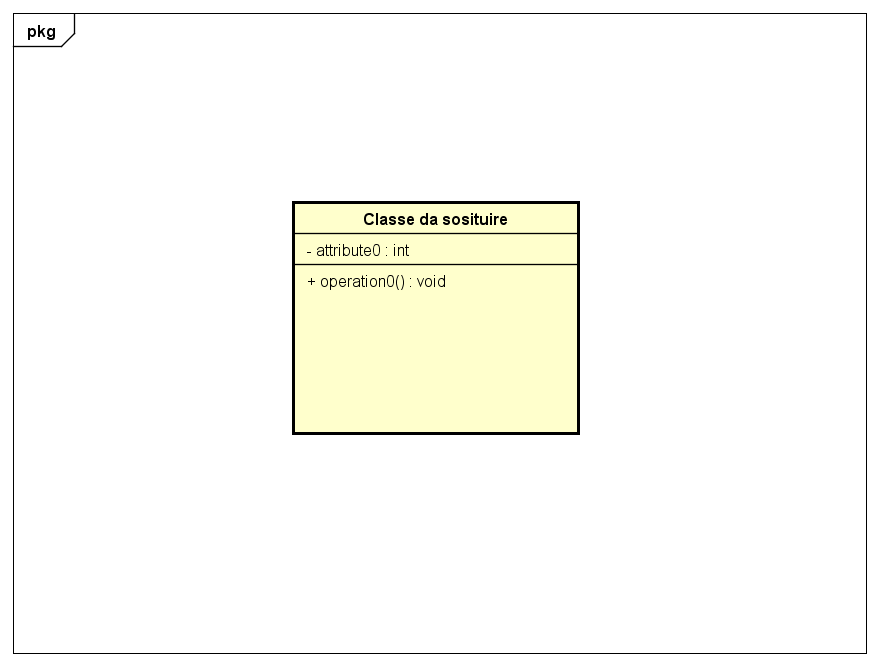
\includegraphics[scale=0.5,keepaspectratio]{UML/Classi/Classi/Temporanea.png}
					\caption{QuizziPedia::Front-End::Templates::}
				\end{figure}
		
			\begin{itemize}
				\item \textbf{Descrizione}: ;
				\item \textbf{Utilizzo}: ;
				\item \textbf{Relazioni con altre classi}: 
				\begin{itemize}
					\item ;
				\end{itemize}
				\item \textbf{Attributi}: 
				\begin{itemize}
					\item ;
				\end{itemize}
				\item \textbf{Metodi}: 
				\begin{itemize}
					\item ;
				\end{itemize}
			\end{itemize}

		\paragraph{QuizziPedia::Front-End::Template::RispostaOrdinamentoImmaginiTemplate}
		
				\label{QuizziPedia::Front-End::Templates::}
				\ref{QuizziPedia::Front-End::Templates::}
				\begin{figure}[h]
					\centering
					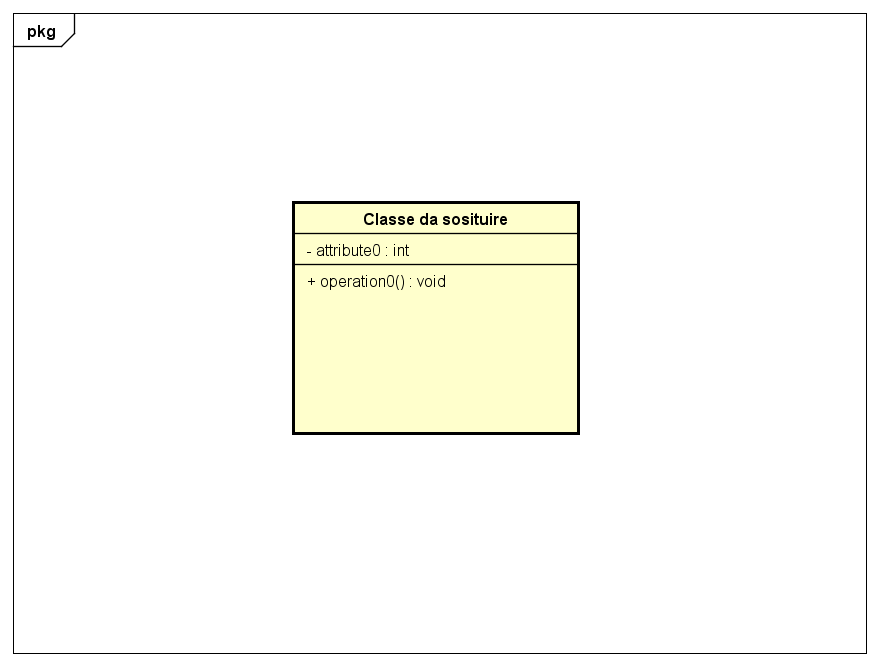
\includegraphics[scale=0.5,keepaspectratio]{UML/Classi/Classi/Temporanea.png}
					\caption{QuizziPedia::Front-End::Templates::}
				\end{figure}
				
			\begin{itemize}
				\item \textbf{Descrizione}: ;
				\item \textbf{Utilizzo}: ;
				\item \textbf{Relazioni con altre classi}: 
				\begin{itemize}
					\item ;
				\end{itemize}
				\item \textbf{Attributi}: 
				\begin{itemize}
					\item ;
				\end{itemize}
				\item \textbf{Metodi}: 
				\begin{itemize}
					\item ;
				\end{itemize}
			\end{itemize}
		
		\paragraph{QuizziPedia::Front-End::Template::RispostaOrdinamentoStringheTemplate}
		
				\label{QuizziPedia::Front-End::Templates::}
				\ref{QuizziPedia::Front-End::Templates::}
				\begin{figure}[h]
					\centering
					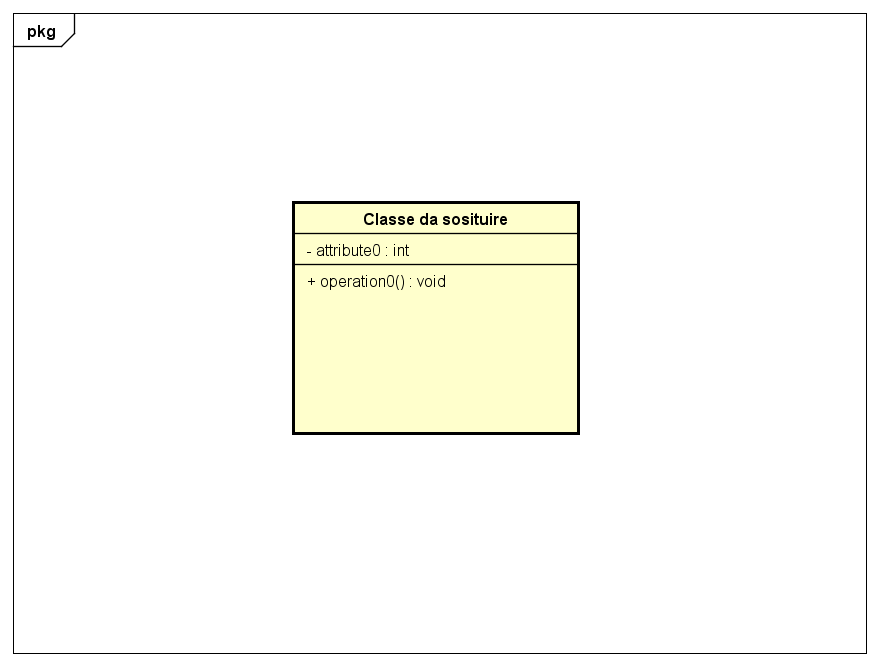
\includegraphics[scale=0.5,keepaspectratio]{UML/Classi/Classi/Temporanea.png}
					\caption{QuizziPedia::Front-End::Templates::}
				\end{figure}
				
			\begin{itemize}
				\item \textbf{Descrizione}: ;
				\item \textbf{Utilizzo}: ;
				\item \textbf{Relazioni con altre classi}: 
				\begin{itemize}
					\item ;
				\end{itemize}
				\item \textbf{Attributi}: 
				\begin{itemize}
					\item ;
				\end{itemize}
				\item \textbf{Metodi}: 
				\begin{itemize}
					\item ;
				\end{itemize}
			\end{itemize}
		
		\paragraph{QuizziPedia::Front-End::Template::RispostaRiempimentoTemplate}
		
				\label{QuizziPedia::Front-End::Templates::}
				\ref{QuizziPedia::Front-End::Templates::}
				\begin{figure}[h]
					\centering
					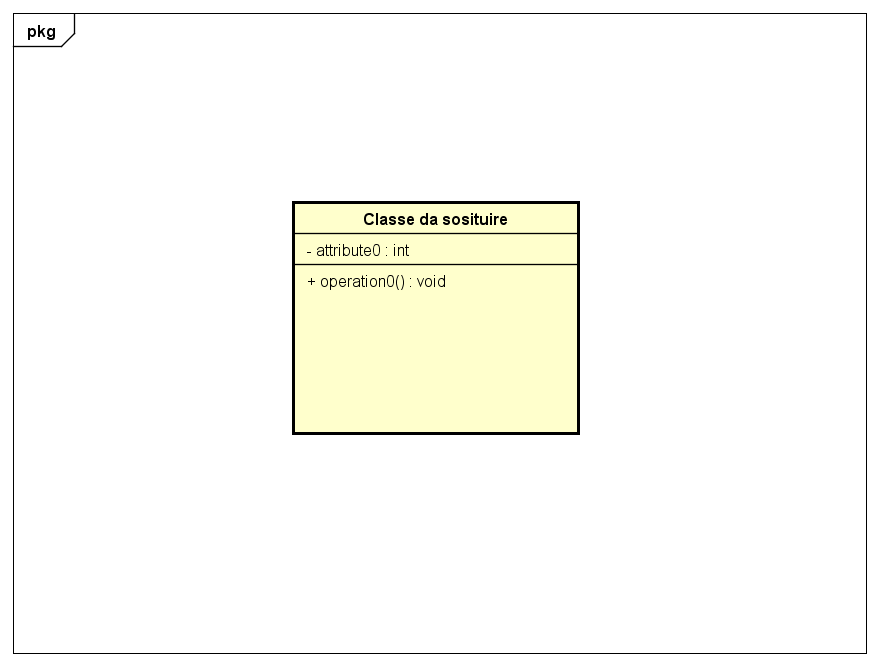
\includegraphics[scale=0.5,keepaspectratio]{UML/Classi/Classi/Temporanea.png}
					\caption{QuizziPedia::Front-End::Templates::}
				\end{figure}
		
			\begin{itemize}
				\item \textbf{Descrizione}: ;
				\item \textbf{Utilizzo}: ;
				\item \textbf{Relazioni con altre classi}: 
				\begin{itemize}
					\item ;
				\end{itemize}
				\item \textbf{Attributi}: 
				\begin{itemize}
					\item ;
				\end{itemize}
				\item \textbf{Metodi}: 
				\begin{itemize}
					\item ;
				\end{itemize}
			\end{itemize}
		
		\paragraph{QuizziPedia::Front-End::Template::RispostaAreaCliccabileTemplate}
		
				\label{QuizziPedia::Front-End::Templates::}
				\ref{QuizziPedia::Front-End::Templates::}
				\begin{figure}[h]
					\centering
					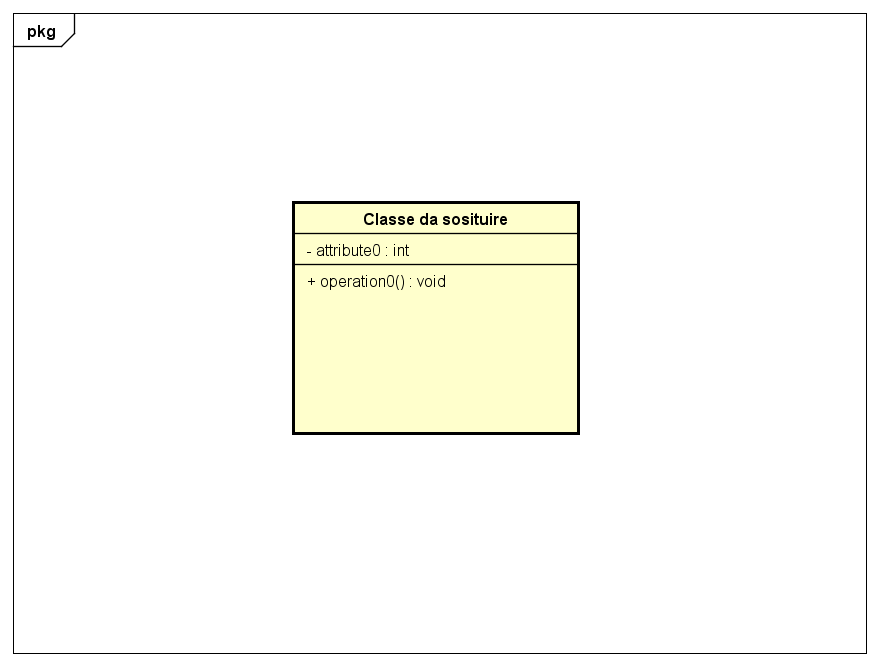
\includegraphics[scale=0.5,keepaspectratio]{UML/Classi/Classi/Temporanea.png}
					\caption{QuizziPedia::Front-End::Templates::}
				\end{figure}
						
			\begin{itemize}
				\item \textbf{Descrizione}: ;
				\item \textbf{Utilizzo}: ;
				\item \textbf{Relazioni con altre classi}: 
				\begin{itemize}
					\item ;
				\end{itemize}
				\item \textbf{Attributi}: 
				\begin{itemize}
					\item ;
				\end{itemize}
				\item \textbf{Metodi}: 
				\begin{itemize}
					\item ;
				\end{itemize}
			\end{itemize}
		
		\paragraph{QuizziPedia::Front-End::Template::RispostaVeroFalsoTemplate}
		
				\label{QuizziPedia::Front-End::Templates::}
				\ref{QuizziPedia::Front-End::Templates::}
				\begin{figure}[h]
					\centering
					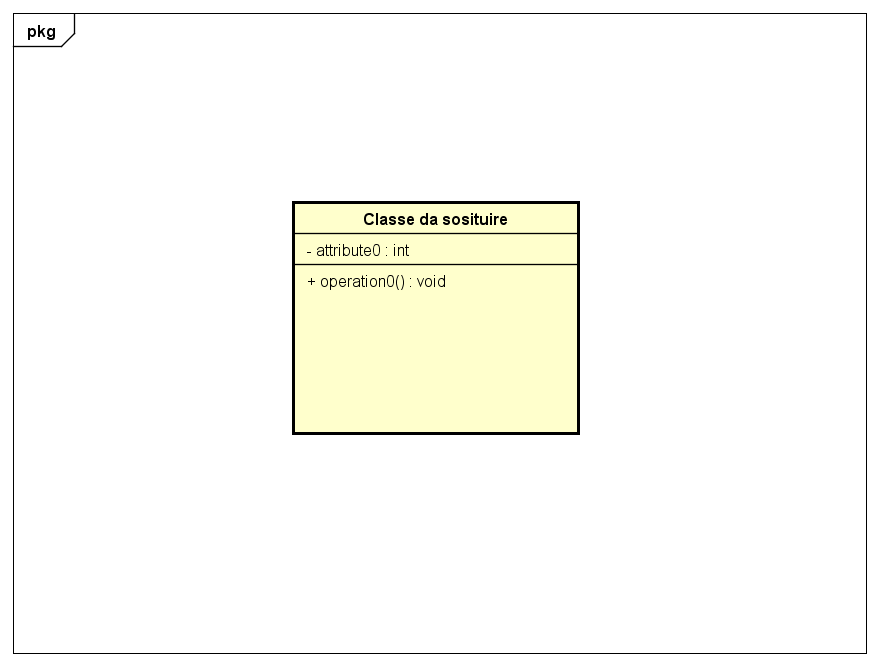
\includegraphics[scale=0.5,keepaspectratio]{UML/Classi/Classi/Temporanea.png}
					\caption{QuizziPedia::Front-End::Templates::}
				\end{figure}
		
			\begin{itemize}
				\item \textbf{Descrizione}: ;
				\item \textbf{Utilizzo}: ;
				\item \textbf{Relazioni con altre classi}: 
				\begin{itemize}
					\item ;
				\end{itemize}
				\item \textbf{Attributi}: 
				\begin{itemize}
					\item ;
				\end{itemize}
				\item \textbf{Metodi}: 
				\begin{itemize}
					\item ;
				\end{itemize}
			\end{itemize}
		
		\paragraph{QuizziPedia::Front-End::Template::RispostaMultiplaTemplate}
		
				\label{QuizziPedia::Front-End::Templates::}
				\ref{QuizziPedia::Front-End::Templates::}
				\begin{figure}[h]
					\centering
					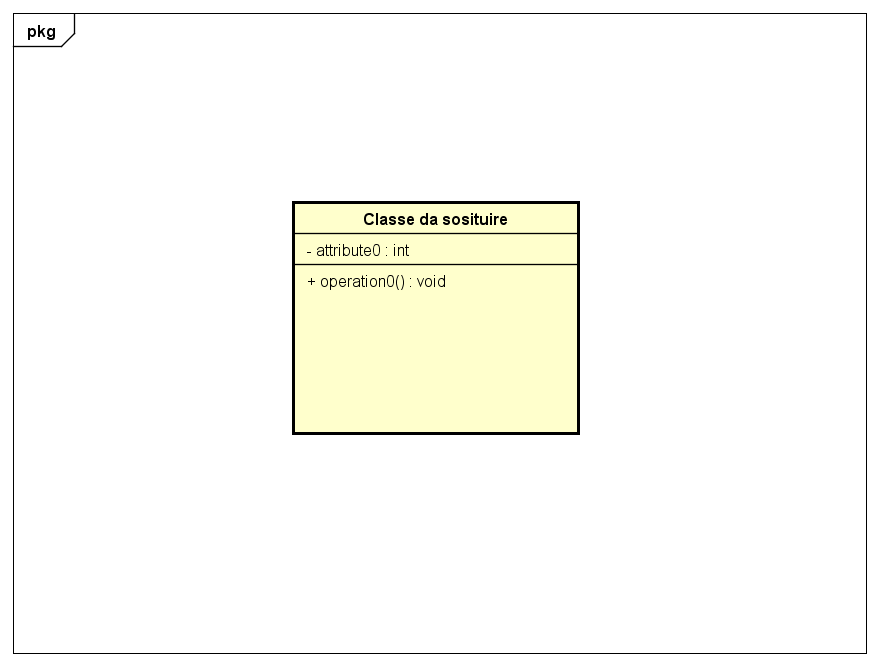
\includegraphics[scale=0.5,keepaspectratio]{UML/Classi/Classi/Temporanea.png}
					\caption{QuizziPedia::Front-End::Templates::}
				\end{figure}		
		
			\begin{itemize}
				\item \textbf{Descrizione}: ;
				\item \textbf{Utilizzo}: ;
				\item \textbf{Relazioni con altre classi}: 
				\begin{itemize}
					\item ;
				\end{itemize}
				\item \textbf{Attributi}: 
				\begin{itemize}
					\item ;
				\end{itemize}
				\item \textbf{Metodi}: 
				\begin{itemize}
					\item ;
				\end{itemize}
			\end{itemize}
		
		\paragraph{QuizziPedia::Front-End::Template::RispostaCollegamentoTemplate}
		
				\label{QuizziPedia::Front-End::Templates::}
				\ref{QuizziPedia::Front-End::Templates::}
				\begin{figure}[h]
					\centering
					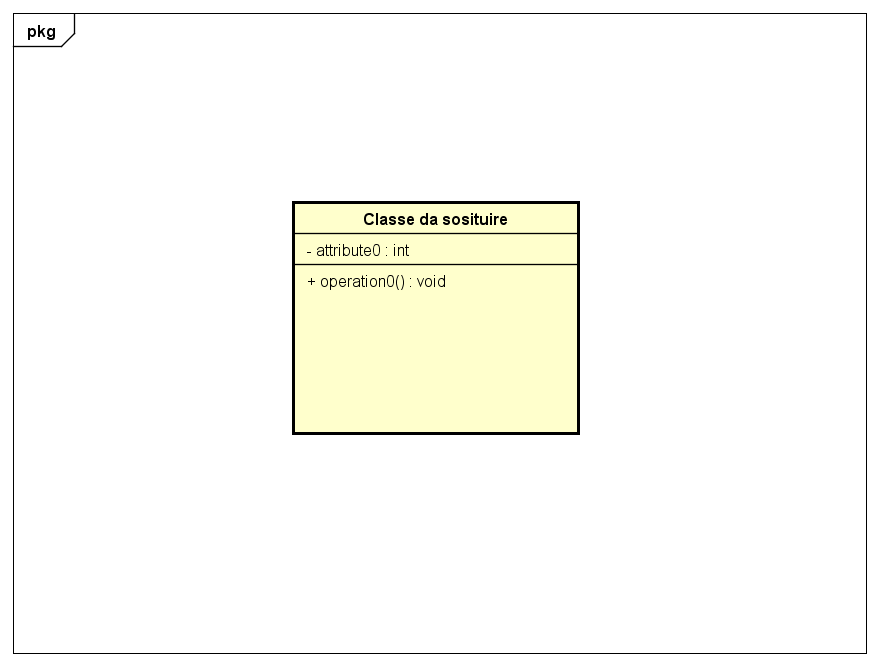
\includegraphics[scale=0.5,keepaspectratio]{UML/Classi/Classi/Temporanea.png}
					\caption{QuizziPedia::Front-End::Templates::}
				\end{figure}
		
			\begin{itemize}
				\item \textbf{Descrizione}: ;
				\item \textbf{Utilizzo}: ;
				\item \textbf{Relazioni con altre classi}: 
				\begin{itemize}
					\item ;
				\end{itemize}
				\item \textbf{Attributi}: 
				\begin{itemize}
					\item ;
				\end{itemize}
				\item \textbf{Metodi}: 
				\begin{itemize}
					\item ;
				\end{itemize}
			\end{itemize}
																					